\chapter{Additional Examples}\label{additional}

This chapter contains additional examples of available methods being applied 
to several test problems. The examples are organized by the test problem
being used. See Section~\ref{intro:files} for help in finding the files referenced
here.

Many of these examples are also used as code verification tests. The examples are
run periodically and the results are checked against known solutions. This 
ensures that the algorithms are correctly implemented. 

\section{Textbook}\label{additional:textbook}

The two-variable version of the ``textbook'' test problem provides
a nonlinearly constrained optimization test case. It is formulated as:
\begin{eqnarray}
\texttt{minimize }
& & f = (x_1-1)^{4}+(x_2-1)^{4}     \nonumber \\
\texttt{subject to }
& & g_1 = x_1^2-\frac{x_2}{2} \le 0 \nonumber \\
& & g_2 = x_2^2-\frac{x_1}{2} \le 0 \label{additional:textbook_f} \\
& &  0.5 \le x_1 \le 5.8            \nonumber \\
& & -2.9 \le x_2 \le 2.9            \nonumber
\end{eqnarray}

Contours of this test problem are illustrated in
Figure~\ref{additional:textbook_prob}(a), with a close-up view of
the feasible region given in
Figure~\ref{additional:textbook_prob}(b).

\begin{figure}[htp!]
  \centering
  \begin{tabular}{cc}
  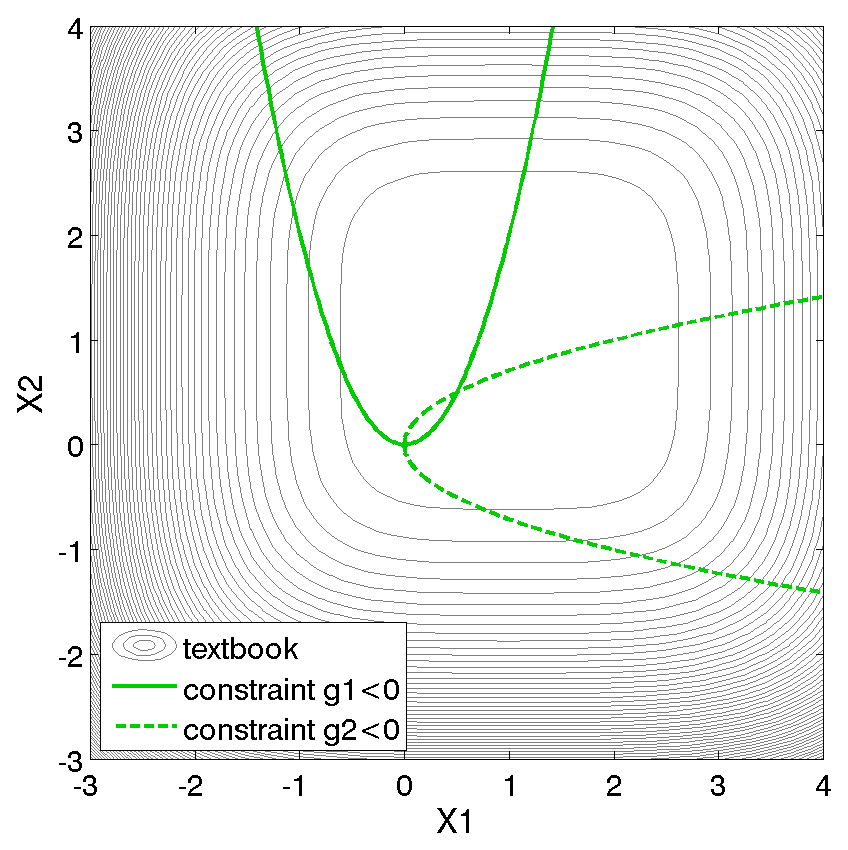
\includegraphics[height=2.5in]{images/textbook_contours} &
  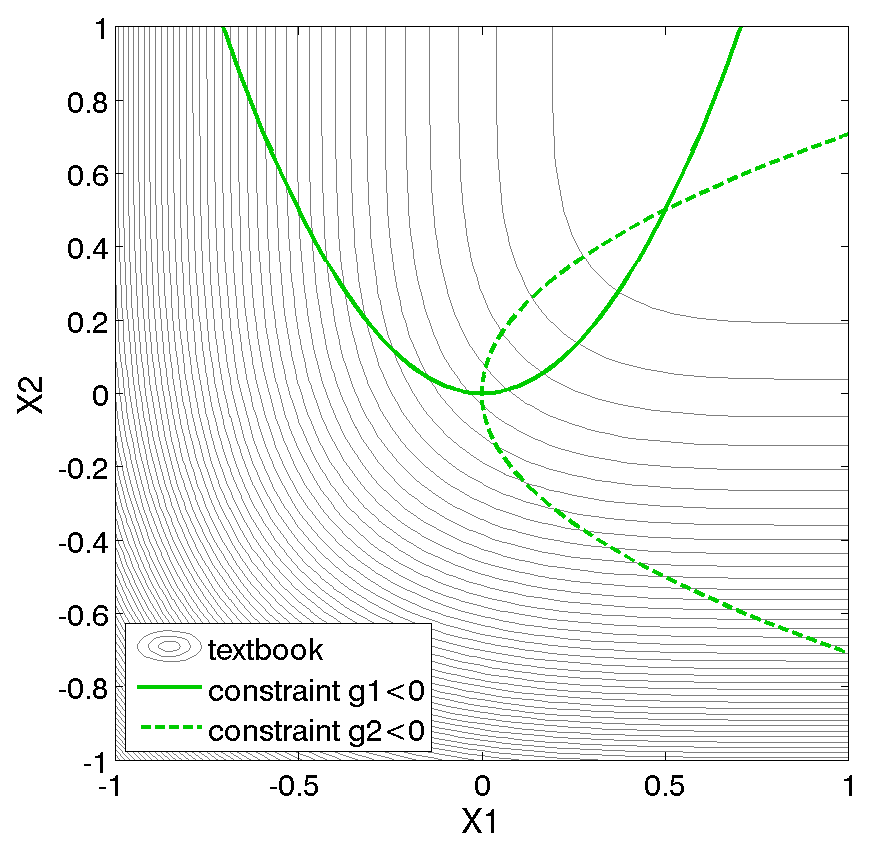
\includegraphics[height=2.5in]{images/textbook_closeup} \\
  (a) & (b) \\
  \end{tabular}
  \caption{Contours of the textbook problem (a) on the $[-3,4] \times
    [-3,4]$ domain and (b) zoomed into an area containing the
    constrained optimum point $(x_1,x_2) = (0.5,0.5)$. The
    feasible region lies at the intersection of the two constraints
    $g_1$ (solid) and $g_2$ (dashed).}
  \label{additional:textbook_prob}
\end{figure}

For the textbook test problem, the unconstrained minimum occurs at
$(x_1,x_2) = (1,1)$. However, the inclusion of the constraints
moves the minimum to $(x_1,x_2) = (0.5,0.5)$.
Equation~\ref{additional:textbook_f} presents the 2-dimensional
form of the textbook problem. An extended formulation is stated as
\begin{eqnarray}
\texttt{minimize }   & & f = \sum_{i=1}^{n}(x_i-1)^4 \nonumber\\
\texttt{subject to } & & g_1 = x_1^2-\frac{x_2}{2} \leq 0
  \label{additional:tbe}\\
  & & g_2=x_2^2-\frac{x_1}{2} \leq 0\nonumber\\
  & & 0.5 \leq x_1 \leq 5.8\nonumber\\
  & & -2.9 \leq x_2 \leq 2.9\nonumber
\end{eqnarray}
where $n$ is the number of design variables. The objective function is
designed to accommodate an arbitrary number of design variables in
order to allow flexible testing of a variety of data sets. Contour
plots for the $n=2$ case have been shown previously in
Figure~\ref{additional:textbook_prob}.

For the optimization problem given in Equation~\ref{additional:tbe}, the
unconstrained solution\\(\texttt{num\_nonlinear\_inequality\_constraints} 
set to zero) for two design variables is:
\begin{eqnarray*}
    x_1 &=& 1.0 \\
    x_2 &=& 1.0
\end{eqnarray*}
with
\begin{eqnarray*}
    f^{\ast} &=& 0.0
\end{eqnarray*}

The solution for the optimization problem constrained by $g_1$\\
(\texttt{num\_nonlinear\_inequality\_constraints} set to one) is:
\begin{eqnarray*}
    x_1 &=& 0.763 \\
    x_2 &=& 1.16
\end{eqnarray*}
with
\begin{eqnarray*}
      f^{\ast} &=& 0.00388 \\
    g_1^{\ast} &=& 0.0 ~~\mathrm{(active)}
\end{eqnarray*}

The solution for the optimization problem constrained by $g_1$ and $g_2$\\
(\texttt{num\_nonlinear\_inequality\_constraints} set to two) is:
\begin{eqnarray*}
    x_1 &=& 0.500 \\
    x_2 &=& 0.500
\end{eqnarray*}
with
\begin{eqnarray*}
      f^{\ast} &=& 0.125 \\
    g_1^{\ast} &=& 0.0 ~~\mathrm{(active)} \\
    g_2^{\ast} &=& 0.0 ~~\mathrm{(active)}
\end{eqnarray*}

Note that as constraints are added, the design freedom is restricted
(the additional constraints are active at the solution) and an
increase in the optimal objective function is observed.

\subsection{Gradient-based Constrained Optimization}\label{additional:textbook:examples:gradient2}

%as of 130124 the example results do NOT match the words in this manual.
%this cannot be fixed without changing the test input file
This example demonstrates the use of a gradient-based optimization
algorithm on a nonlinearly constrained problem. The 
Dakota input file for this example is
shown in Figure~\ref{additional:textbook_grad_constr}. This
input file is similar to the input file for the unconstrained
gradient-based optimization example involving the Rosenbrock
function, seen in Section~\ref{tutorial:examples:optimization}. 
Note the addition of commands in the responses block of
the input file that identify the number and type of constraints, along
with the upper bounds on these constraints. The commands
\texttt{direct} and \texttt{analysis\_driver = 'text\_book'} specify
that Dakota will use its internal version of the textbook problem.

\begin{figure}[ht!]
  \centering
  \begin{bigbox}
    \begin{small}
      \verbatimtabinput[8]{textbook_opt_conmin.in}
    \end{small}
  \end{bigbox}
  \caption{Textbook gradient-based constrained optimization example:
    the Dakota input file --
see \texttt{Dakota/examples/users/textbook\_opt\_conmin.in} }
  \label{additional:textbook_grad_constr}
\end{figure}

The \texttt{conmin\_mfd} keyword in
Figure~\ref{additional:textbook_grad_constr} tells Dakota to use the
CONMIN package's implementation of the Method of Feasible Directions
(see Section~\ref{opt:methods:gradient:descriptions} for more
details).

A significantly faster alternative is the DOT package's Modified
Method of Feasible Directions, i.e. \texttt{dot\_mmfd} (see
Section~\ref{opt:methods:gradient:descriptions} for more
details). However, DOT is licensed software that may not be available
on a particular system. If it is installed on your system and Dakota
has been compiled without the \texttt{--without-dot} flag, you may use
it by commenting out the line with \texttt{conmin\_mfd} and
uncommenting the line with \texttt{dot\_mmfd}.

The results of the optimization example are listed at the end of
the output file (see Section~\ref{tutorial:quickstart:output}.
This information shows that the
optimizer stopped at the point $(x_1,x_2) = (0.5,0.5)$, where both
constraints are approximately satisfied, and where the objective function value is
$0.128$. The progress of the optimization algorithm is shown in
Figure~\ref{additional:textbook_grad_constr_graphics}(b) where the
dots correspond to the end points of each iteration in the algorithm. The
starting point is $(x_1,x_2) = (0.9,1.1)$, where both constraints
are violated. The optimizer takes a
sequence of steps to minimize the objective function while reducing
the infeasibility of the constraints.
The optimization graphics are also shown in
Figure~\ref{additional:textbook_grad_constr_graphics}(a).

\begin{figure}[ht!]
  \centering
  \begin{tabular}{c}
  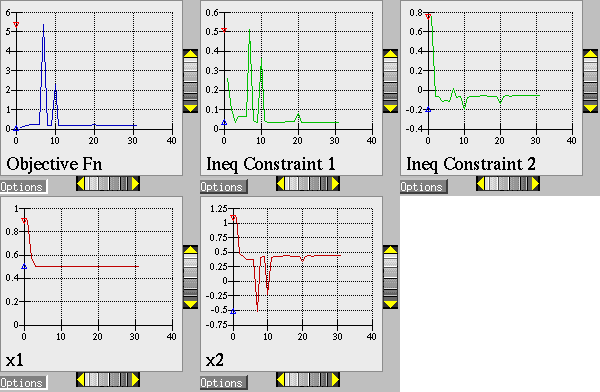
\includegraphics[width=\textwidth]{images/textbook_opt_hist}\\
  (a)\\
  \qquad\\
  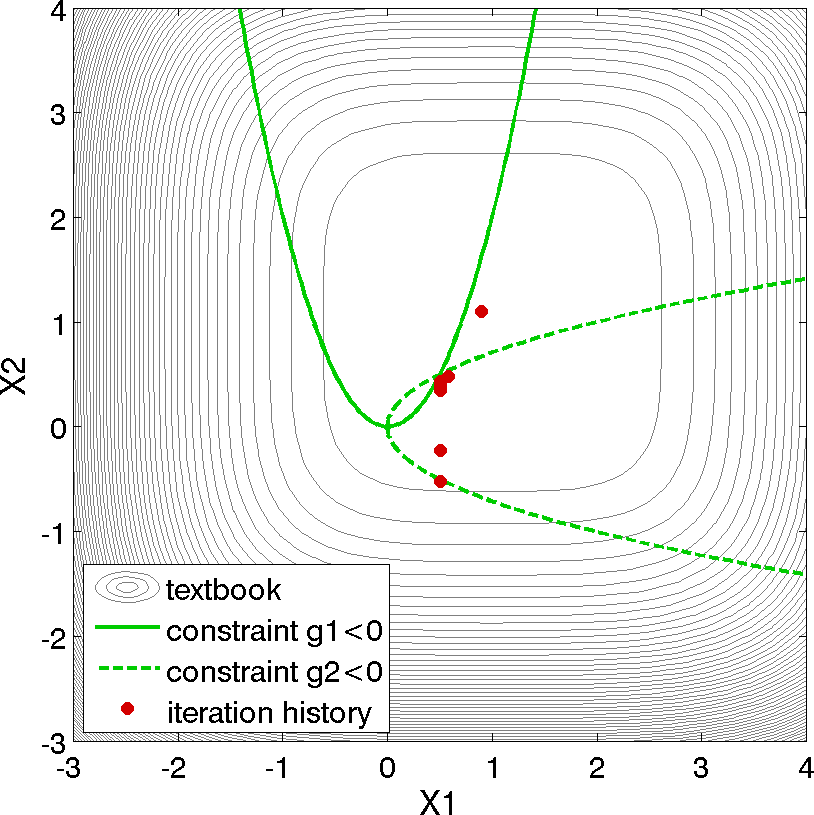
\includegraphics[height=2.5in]{images/textbook_history} \\
  (b)
  \end{tabular}
  \caption{Textbook gradient-based constrained optimization example:
    (a) screen capture of the Dakota graphics shows how the objective
    function was reduced during the search for a feasible design point
    and (b) iteration history (iterations marked by solid dots).}
  \label{additional:textbook_grad_constr_graphics}
\end{figure}

% \subsection{Least Squares Optimization}\label{additional:textbook:least}
% 
%khu 130124 - I don't see the point of this example.  it is confusing because
%the formulation changes and the solution changes. it also replicates the
%example w/ the Rosenbrock test function.
% This test problem may also be used to exercise least squares
% solution methods by modifying the problem formulation to:
% \begin{equation}
% \texttt{minimize } (f)^2+(g_1)^2+(g_2)^2 \label{additional:tbls}
% \end{equation}
% 
% This modification is performed by simply changing the responses
% specification for the three functions from
% \texttt{num\_objective\_functions = 1} and
% \texttt{num\_nonlinear\_inequality\_constraints = 2} to \\
% \texttt{num\_least\_squares\_terms = 3}. Note that the two problem
% formulations are not equivalent and have different solutions.
% 
% % Another way to exercise the least squares methods which would be
% % equivalent to the optimization formulation would be to select the
% % residual functions to be $(x_{i}-1)^2$. However, this formulation
% % requires modification to \texttt{Dakota\_Source/test/text\_book.cpp} and will
% % not be presented here. Equation~\ref{additional:tbls}, on the other
% % hand, can use the existing \texttt{text\_book} without modification.
% Refer to Section~\ref{additional:rosenbrock} for an example of
% minimizing the same objective function using both optimization and
% least squares approaches.
% 
% The solution for the least squares problem given in 
% Equation~\ref{additional:tbls} is:
% \begin{eqnarray*}
%     x_1 &=& 0.566 \\
%     x_2 &=& 0.566
% \end{eqnarray*}
% with the residual functions equal to
% \begin{eqnarray*}
%       f^{\ast} &=& 0.0713 \\
%     g_1^{\ast} &=& 0.0371 \\
%     g_2^{\ast} &=& 0.0371
% \end{eqnarray*}
% and a minimal sum of the squares of $0.00783$.
% 
% This study requires selection of \texttt{num\_least\_squares\_terms = 3} 
% in the responses specification and selection of either 
% \texttt{optpp\_g\_newton}, \texttt{nlssol\_sqp}, or \texttt{nl2sol} in 
% the method specification.

\clearpage
\section{Rosenbrock}\label{additional:rosenbrock}

The Rosenbrock function~\cite{Gil81} is a well known test problem
for optimization algorithms. The standard formulation includes two design variables,
and computes a single objective function.
%however, additional formulations have been proposed to test algorithm performance in
%higher dimensions. 
This problem can also be posed as a least-squares optimization 
problem with two residuals to be minimzed because the objective 
function is the sum of squared terms.


{\bf Standard Formulation} \\
The standard two-dimensional formulation can be stated as
\begin{equation}
\texttt{minimize } f=100(x_2-x_1^2)^2+(1-x_1)^2 \label{additional:rosenstd}
\end{equation}

Surface and contour plots for this function have been shown previously
in Figure~\ref{tutorial:rosenbrock_prob}. 

The optimal solution is:
\begin{eqnarray*}
    x_1 &=& 1.0 \\
    x_2 &=& 1.0
\end{eqnarray*}
with
\begin{eqnarray*}
    f^{\ast} &=& 0.0
\end{eqnarray*}

A discussion of gradient based optimization to minimize 
this function is in Section~\ref{tutorial:examples:optimization}.

% {\bf ``Extended'' Formulation} \\
% The formulation in \cite{Noc99} is called the ``extended Rosenbrock'' and is defined as:
% \begin{equation}
% f = \sum_{i=1}^{n/2} \left[ \alpha (x_{2i}-x_{2i-1}^2)^2+(1-x_{2i-1})^2 \right]
% \label{additional:rosenexd}
% \end{equation}
% 
% {\bf ``Generalized'' Formulation} \\
% Another n-dimensional formulation was propsed in~\cite{Sch87}.
% \begin{equation}
% f = \sum_{i=1}^{n-1} \left[ 100 (x_{i+1}-x_i^2)^2+(1-x_i)^2 \right]
% \label{additional:rosengen}
% \end{equation}
% 
% \begin{equation}
% f = \sum_{i=1}^{n/2} \left[ e^{-x^2_{2i-1}} + 10 e^{-x^2_{2i}} \right]
% \label{additional:gerstner_aniso1}
% \end{equation}
% \begin{equation}
% f = exp\left(-\sum_{i=1}^{n/2} \left[ 10 x^2_{2i-1} + 5 x^2_{2i} \right]\right)
% \label{additional:gerstner_aniso3}
% \end{equation}

{\bf A Least-Squares Optimization Formulation} \\
This test problem
may also be used to exercise least-squares solution methods by
recasting the standard problem formulation into:
\begin{equation}
\texttt{minimize } f = (f_1)^2+(f_2)^2 \label{additional:rosenls}
\end{equation}
where
\begin{equation}
f_1 = 10 (x_2 - x_1^2) \label{additional:rosenr1}
\end{equation}
and
\begin{equation}
f_2 = 1 - x_1 \label{additional:rosenr2}
\end{equation}
are residual terms.

The included analysis driver can handle both formulations.
In the \texttt{Dakota/test} directory, the \texttt{rosenbrock}
executable (compiled from \texttt{Dakota\_Source/test/rosenbrock.cpp}) checks the number of
response functions passed in the parameters file and returns either an
objective function (as computed from
Equation~\ref{additional:rosenstd}) for use with optimization methods
or two least squares terms (as computed from
Equations~\ref{additional:rosenr1}-\ref{additional:rosenr2}) for use
with least squares methods. Both cases support analytic gradients of
the function set with respect to the design variables.
See Figure~\ref{tutorial:rosenbrock_grad} (std formulation) 
and Figure~\ref{additional:rosenbrock_nls} (least squares formulation)
for examples of each usage.


% \subsection{Optimization Results}\label{additional:rosenbrock:results}
% 
%khu this belongs in a methods section
% In comparing the two approaches, one would expect the Gauss-Newton
% approach to be more efficient since it exploits the special-structure
% of a least squares objective function and, in this problem, the
% Gauss-Newton Hessian is a good approximation since the least squares
% residuals are zero at the solution. From a good initial guess, this
% expected behavior is clearly demonstrated. Starting from
% \texttt{cdv\_initial\_point = 0.8, 0.7}, the \texttt{optpp\_g\_newton}
% method converges in only 3 function and gradient evaluations while the
% \texttt{optpp\_q\_newton} method requires 27 function and gradient
% evaluations to achieve similar accuracy. Starting from a poorer
% initial guess (e.g., \texttt{cdv\_initial\_point = -1.2, 1.0}), the
% trend is less obvious since both methods spend several evaluations
% finding the vicinity of the minimum (total function and gradient
% evaluations = 45 for \texttt{optpp\_q\_newton} and 29 for
% \texttt{optpp\_g\_newton}). However, once the vicinity is located and
% the Hessian approximation becomes accurate, convergence is much more
% rapid with the Gauss-Newton approach.
% 
% Shown below is the complete Dakota output for the
% \texttt{optpp\_g\_newton} method starting from\\
% \texttt{cdv\_initial\_point = 0.8, 0.7}:
% \begin{small}
% \begin{verbatim}
% Running MPI executable in serial mode.
% Dakota version 6.0 release.
% Subversion revision xxxx built May ...
% Writing new restart file dakota.rst
% gradientType = analytic
% hessianType = none
% 
% >>>>> Executing environment.
% 
% >>>>> Running optpp_g_newton iterator.
% 
% ------------------------------
% Begin Function Evaluation    1
% ------------------------------
% Parameters for function evaluation 1:
%                       8.0000000000e-01 x1
%                       7.0000000000e-01 x2
% 
% rosenbrock /tmp/file4t29aW /tmp/filezGeFpF
% 
% Active response data for function evaluation 1:
% Active set vector = { 3 3 } Deriv vars vector = { 1 2 }
%                       6.0000000000e-01 least_sq_term_1
%                       2.0000000000e-01 least_sq_term_2
%  [ -1.6000000000e+01  1.0000000000e+01 ] least_sq_term_1 gradient
%  [ -1.0000000000e+00  0.0000000000e+00 ] least_sq_term_2 gradient
% 
% 
% 
% 
% ------------------------------
% Begin Function Evaluation    2
% ------------------------------
% Parameters for function evaluation 2:
%                       9.9999528206e-01 x1
%                       9.5999243139e-01 x2
% 
% rosenbrock /tmp/fileSaxQHo /tmp/fileHnU1Z7
% 
% Active response data for function evaluation 2:
% Active set vector = { 3 3 } Deriv vars vector = { 1 2 }
%                      -3.9998132761e-01 least_sq_term_1
%                       4.7179363810e-06 least_sq_term_2
%  [ -1.9999905641e+01  1.0000000000e+01 ] least_sq_term_1 gradient
%  [ -1.0000000000e+00  0.0000000000e+00 ] least_sq_term_2 gradient
% 
% 
% 
% 
% ------------------------------
% Begin Function Evaluation    3
% ------------------------------
% Parameters for function evaluation 3:
%                       9.9999904377e-01 x1
%                       9.9999808276e-01 x2
% 
% rosenbrock /tmp/filedtRtlR /tmp/file3kUVGA
% 
% Active response data for function evaluation 3:
% Active set vector = { 3 3 } Deriv vars vector = { 1 2 }
%                      -4.7950734494e-08 least_sq_term_1
%                       9.5622502239e-07 least_sq_term_2
%  [ -1.9999980875e+01  1.0000000000e+01 ] least_sq_term_1 gradient
%  [ -1.0000000000e+00  0.0000000000e+00 ] least_sq_term_2 gradient
% 
% 
% 
% 
% ------------------------------
% Begin Function Evaluation    4
% ------------------------------
% Parameters for function evaluation 4:
%                       9.9999904377e-01 x1
%                       9.9999808276e-01 x2
% 
% Duplication detected: analysis_drivers not invoked.
% 
% Active response data retrieved from database:
% Active set vector = { 2 2 } Deriv vars vector = { 1 2 }
%  [ -1.9999980875e+01  1.0000000000e+01 ] least_sq_term_1 gradient
%  [ -1.0000000000e+00  0.0000000000e+00 ] least_sq_term_2 gradient
% 
% 
% <<<<< Function evaluation summary: 4 total (3 new, 1 duplicate)
% <<<<< Best parameters          =
%                       9.9999904377e-01 x1
%                       9.9999808276e-01 x2
% <<<<< Best residual norm =  9.5742653315e-07; 0.5 * norm^2 =  4.5833278319e-13
% <<<<< Best residual terms      =
%                      -4.7950734494e-08
%                       9.5622502239e-07
% <<<<< Best data captured at function evaluation 3
% Confidence Interval for x1 is [  9.9998687852e-01,  1.0000112090e+00 ]
% Confidence Interval for x2 is [  9.9997372187e-01,  1.0000224436e+00 ]
% 
% <<<<< Iterator optpp_g_newton completed.
% <<<<< Environment execution completed.
% Dakota execution time in seconds:
%   Total CPU        =       0.01 [parent =   0.017997, child =  -0.007997]
%   Total wall clock =  0.0672231
% \end{verbatim}
% \end{small}

\subsection{Least-Squares Optimization}\label{additional:rosenbrock:examples:nonlinear}

Least squares methods are often used for calibration or parameter
estimation, that is, to seek parameters maximizing agreement of models
with experimental data. The least-squares formulation was described in 
the previous section.

When using a least-squares approach to minimize a function, each of the
least-squares terms $f_1, f_2,\ldots$ is driven toward zero. This
formulation permits the use of specialized algorithms that can be more
efficient than general purpose optimization algorithms. See
Chapter~\ref{nls} for more detail on the algorithms used for least-squares
minimization, as well as a discussion on the types of
engineering design problems (e.g., parameter estimation) that can make
use of the least-squares approach.

Figure~\ref{additional:rosenbrock_nls} is a listing of the Dakota input
file \texttt{rosen\_opt\_nls.in}. This differs from the input
file shown in Figure~\ref{tutorial:rosenbrock_grad} in several key
areas. The responses block of the input file uses the keyword
\texttt{calibration\_terms = 2} instead of
\texttt{objective\_functions = 1}.
%The keywords in the interface block show that the Unix fork method
%is used to run the C++ analysis code named \texttt{rosenbrock}.
The method block of the input file shows that the NL2SOL
algorithm~\cite{Den81} (\texttt{nl2sol}) is used in this example. (The
Gauss-Newton, NL2SOL, and NLSSOL SQP algorithms are currently
available for exploiting the special mathematical structure of least
squares minimization problems).

\begin{figure}[ht!]
  \centering
  \begin{bigbox}
    \begin{small}
      \verbatimtabinput[8]{rosen_opt_nls.in}
    \end{small}
  \end{bigbox}
  \caption{Rosenbrock nonlinear least squares example: the Dakota input file --
see \texttt{Dakota/examples/users/rosen\_opt\_nls.in} }
  \label{additional:rosenbrock_nls}
\end{figure}

The optimization results at the end of the output file show that the least
squares minimization approach has found the same optimum design point,
$(x1,x2) = (1.0,1.0)$, as was found using the conventional
gradient-based optimization approach. The iteration history of the
least squares minimization is given in
Figure~\ref{additional:rosenbrock_nls_graphics}, and shows that 14
function evaluations were needed for convergence. In this example the
least squares approach required about half the number of function
evaluations as did conventional gradient-based optimization.
In many cases a good least squares algorithm will converge more rapidly
in the vicinity of the solution.

\begin{figure}[ht!]
  \centering
  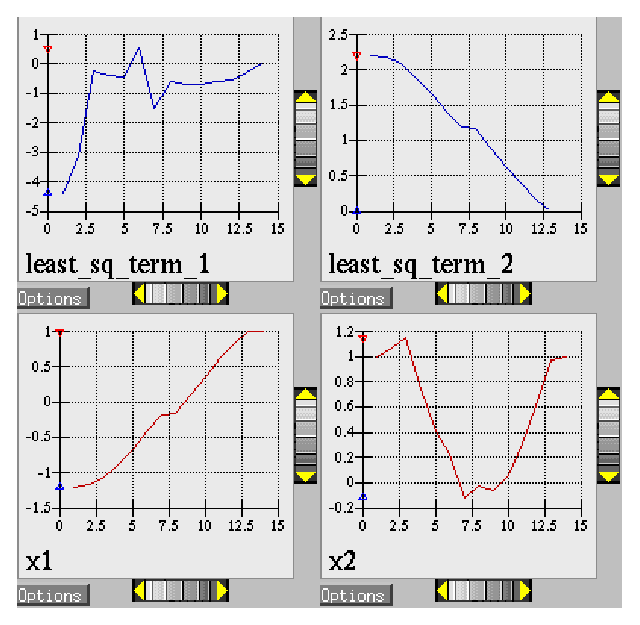
\includegraphics[height=4in]{images/nonlin_paramest_hist}
  \caption{Rosenbrock nonlinear least squares example: iteration
    history for least squares terms $f_1$ and $f_2$.}
  \label{additional:rosenbrock_nls_graphics}
\end{figure}

\clearpage
\section{Herbie, Smooth Herbie, and Shubert}
% need to update citation from ToAppear to a date when it does appear 
Lee, et al. \cite{herbiefunc} developed the Herbie function as a 2D
test problem for surrogate-based optimization. However, since it is
separable and each dimension is identical it is easily generalized to
an arbitrary number of dimensions. The generalized (to $M$
dimensions) Herbie function is
\begin{displaymath}
{\rm herb}(\underline{x})=-\prod_{k=1}^M w_{herb}\left(x_k\right)
\end{displaymath}
where 
\begin{displaymath}
w_{herb}\left(x_k\right)=\exp(-(x_k-1)^2)+\exp(-0.8(x_k+1)^2)-0.05\sin\left(8\left(x_k+0.1\right)\right).
\end{displaymath}
The Herbie function's high frequency sine component creates a large
number of local minima and maxima, making it a significantly more
challenging test problem. However, when testing a method's ability to
exploit smoothness in the true response, it is desirable to have a
less oscillatory function. For this reason, the ``smooth Herbie''
test function omits the high frequency sine term but is otherwise
identical to the Herbie function. The formula for smooth Herbie is
\begin{displaymath}
{\rm herb_{sm}}(\underline{x})=-\prod_{k=1}^M w_{sm}\left(x_k\right)
\end{displaymath}
where 
\begin{displaymath}
w_{sm}\left(x_k\right)=\exp(-(x_k-1)^2)+\exp(-0.8(x_k+1)^2).
\end{displaymath}
Two dimensional versions of the \texttt{herbie} and \texttt{smooth\_herbie} 
test functions are plotted in Figure~\ref{fig:2D_herbie__smooth_herbie}.
\begin{figure}[hbp]
  \centering
  \centerline{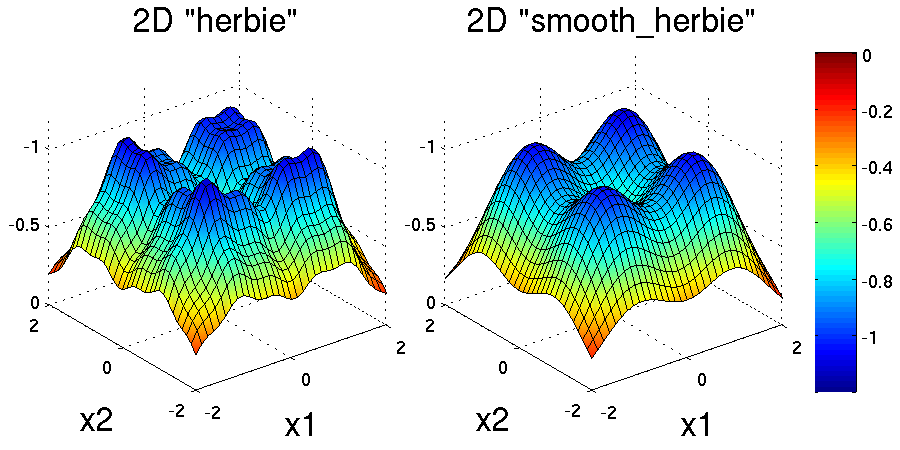
\includegraphics[scale=1.0]{images/DAK5pt2_2D__herbie__smooth_herbie}}
  \caption{Plots of the \texttt{herbie} (left) and
           \texttt{smooth\_herbie} (right) test functions in 2
           dimensions. They can accept an arbitrary number of
           inputs. The direction of the z-axis has been reversed 
           (negative is up) to better view the functions' minima.}
  \label{fig:2D_herbie__smooth_herbie}
\end{figure}

Shubert is another separable (and therefore arbitrary dimensional) 
test function. Its analytical formula is
\begin{eqnarray*}
{\rm shu}(\underline{x})= \prod_{k=1}^M w_{shu}\left(x_k\right) \\
w_{shu}\left(x_k\right)= \sum_{i=1}^5 i\cos((i+1)x_k+i)
\end{eqnarray*}
The 2D version of the \texttt{shubert} function is shown in 
Figure~\ref{fig:2D_shubert}. 

\subsection{Efficient Global Optimization}

The Dakota input file \texttt{herbie\_shubert\_opt\_ego.in} shows how
to use efficient global optimization (ego) to minimize the 5D version
of any of these 3 separable functions. The input file is shown in 
Figure~\ref{additional:herbie_shubert_ego}. Note that in the variables
section the \texttt{5*} preceding the values -2.0 and 2.0 for the
\texttt{lower\_bounds} and \texttt{upper\_bounds}, respectively, tells
Dakota to repeat them 5 times. The ``interesting'' region for each 
of these functions is $-2\le x_k \le 2$ for all dimensions.

\begin{figure}[ht!]
  \centering
  \begin{small}
    \begin{bigbox}
      \verbatimtabinput[8]{herbie_shubert_opt_ego.in}
    \end{bigbox}
  \end{small}
  \caption{Herbie/Shubert examples: the Dakota input file --
see \texttt{Dakota/examples/users/herbie\_shubert\_opt\_ego.in} }
  \label{additional:herbie_shubert_ego}
\end{figure}

\begin{figure}
  \centering
  \centerline{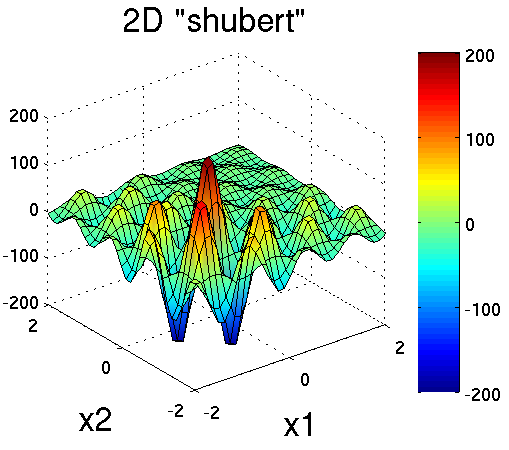
\includegraphics[scale=1.0]{images/DAK5pt2_2D_shubert}}
  \caption{Plot of the \texttt{shubert} test function in 2 dimensions.
           It can accept an arbitrary number of inputs.}
  \label{fig:2D_shubert}
\end{figure}

%\clearpage
\section{Cylinder Head}\label{additional:cylinder}

The cylinder head test problem is stated as:
\begin{eqnarray}
\texttt{minimize }   & & f=-1\bigg(\frac{\mathtt{horsepower}}{250}+
  \frac{\mathtt{warranty}}{100000}\bigg) \nonumber\\
\texttt{subject to } & & \sigma_{max} \leq 0.5 \sigma_{yield}
  \label{additional:cylhead}\\
                     & & \mathtt{warranty} \geq 100000          \nonumber\\
                     & & \mathtt{time_{cycle}} \leq 60          \nonumber\\
                     & & 1.5 \leq \mathtt{d_{intake}} \leq 2.164\nonumber\\
                     & & 0.0 \leq \mathtt{flatness} \leq 4.0    \nonumber
\end{eqnarray}

This formulation seeks to simultaneously maximize normalized engine
horsepower and engine warranty over variables of valve intake diameter
($\mathtt{d_{intake}}$) in inches and overall head flatness
($\mathtt{flatness}$) in thousandths of an inch subject to inequality
constraints that the maximum stress cannot exceed half of yield, that
warranty must be at least 100000 miles, and that manufacturing cycle
time must be less than 60 seconds. Since the constraints involve
different scales, they should be nondimensionalized (note: the
nonlinear constraint scaling described in
Section~\ref{opt:additional:scaling} can now do this
automatically). In addition, they can be converted to the standard
1-sided form $g(\mathbf{x}) \leq 0$ as follows:
\begin{eqnarray}
  & & g_1=\frac{2\sigma_{\mathtt{max}}}{\sigma_{\mathtt{yield}}}-1 \leq 0
  \nonumber\\
  & & g_2=1-\frac{\mathtt{warranty}}{100000} \leq 0
  \label{additional:cylheadaltg}\\
  & & g_3=\frac{\mathtt{time_{cycle}}}{60}-1 \leq 0\nonumber
\end{eqnarray}

The objective function and constraints are related analytically to the
design variables according to the following simple expressions:
\begin{eqnarray}
\mathtt{warranty}     &=& 100000+15000(4-\mathtt{flatness})\nonumber\\
\mathtt{time_{cycle}} &=& 45+4.5(4-\mathtt{flatness})^{1.5}\nonumber\\
\mathtt{horsepower}   &=& 250+200\bigg(\frac{\mathtt{d_{intake}}}{1.833}-1\bigg)
  \label{additional:cylheadexp}\\
\sigma_{\mathtt{max}} &=& 750+\frac{1}{(\mathtt{t_{wall}})^{2.5}}\nonumber\\
\mathtt{t_{wall}}     &=& \mathtt{offset_{intake}-offset_{exhaust}}-
  \frac{(\mathtt{d_{intake}-d_{exhaust}})}{2}\nonumber
\end{eqnarray}

where the constants in Equation~\ref{additional:cylheadaltg} and
Equation~\ref{additional:cylheadexp} assume the following values:
$\sigma_{\mathtt{yield}}=3000$, $\mathtt{offset_{intake}}=3.25$,
$\mathtt{offset_{exhaust}}=1.34$, and $\mathtt{d_{exhaust}}=1.556$.

\subsection{Constrained Gradient Based Optimization}

An example using the cylinder head test problem is shown below:
\begin{figure}[ht!]
  \centering
  \begin{small}
    \begin{bigbox}
      \verbatimtabinput[8]{cylhead_opt_npsol.in}
    \end{bigbox}
  \end{small}
  \caption{Cylinder Head Example: the Dakota input file --
see \texttt{Dakota/examples/users/cylhead\_opt\_npsol.in} }
  \label{additional:cylinder_head}
\end{figure}

The interface keyword specifies use of the \texttt{cyl\_head}
executable (compiled from \texttt{Dakota\_Source/test/cyl\_head.cpp}) as the
simulator. The variables and responses keywords specify the data sets
to be used in the iteration by providing the initial point,
descriptors, and upper and lower bounds for two continuous design
variables and by specifying the use of one objective function, three
inequality constraints, and numerical gradients in the problem. The
method keyword specifies the use of the \texttt{npsol\_sqp} method to
solve this constrained optimization problem. No environment keyword is
specified, so the default \texttt{single\_method} approach is used.

The solution for the constrained optimization problem is:
\begin{eqnarray*}
    \mathrm{intake\_dia} &=& 2.122 \\
    \mathrm{flatness}    &=& 1.769
\end{eqnarray*}
with
\begin{eqnarray*}
      f^{\ast} &=& -2.461 \\
    g_1^{\ast} &=&  0.0    ~~\mathrm{(active)} \\
    g_2^{\ast} &=& -0.3347 ~~\mathrm{(inactive)} \\
    g_3^{\ast} &=&  0.0    ~~\mathrm{(active)}
\end{eqnarray*}
which corresponds to the following optimal response quantities:
\begin{eqnarray*}
    \mathrm{warranty}        &=& 133472 \\
    \mathrm{cycle\_time}     &=& 60 \\
    \mathrm{wall\_thickness} &=& 0.0707906 \\
    \mathrm{horse\_power}    &=& 281.579 \\
    \mathrm{max\_stress}     &=& 1500
\end{eqnarray*}

The final report from the Dakota output is as follows:
\begin{small}
\begin{verbatim}
    <<<<< Iterator npsol_sqp completed.					 
    <<<<< Function evaluation summary: 55 total (55 new, 0 duplicate)	 
    <<<<< Best parameters          =					 
                          2.1224188322e+00 intake_dia			 
                          1.7685568331e+00 flatness
    <<<<< Best objective function  =					 
                         -2.4610312954e+00
    <<<<< Best constraint values   =		 
                          1.8407497748e-13
                         -3.3471647504e-01
                          0.0000000000e+00
    <<<<< Best data captured at function evaluation 51
    <<<<< Environment execution completed.
    Dakota execution time in seconds:					 
      Total CPU        =       0.04 [parent =   0.031995, child =   0.008005]
      Total wall clock =   0.232134
\end{verbatim}
\end{small}

\clearpage
\section{Container}\label{additional:container}

For this example, suppose that a high-volume manufacturer of light
weight steel containers wants to minimize the amount of raw sheet
material that must be used to manufacture a 1.1 quart
cylindrical-shaped can, including waste material. Material for the
container walls and end caps is stamped from stock sheet material of
constant thickness. The seal between the end caps and container wall
is manufactured by a press forming operation on the end caps. The end
caps can then be attached to the container wall forming a seal through
a crimping operation.

\begin{figure}[hb]
  \centering
  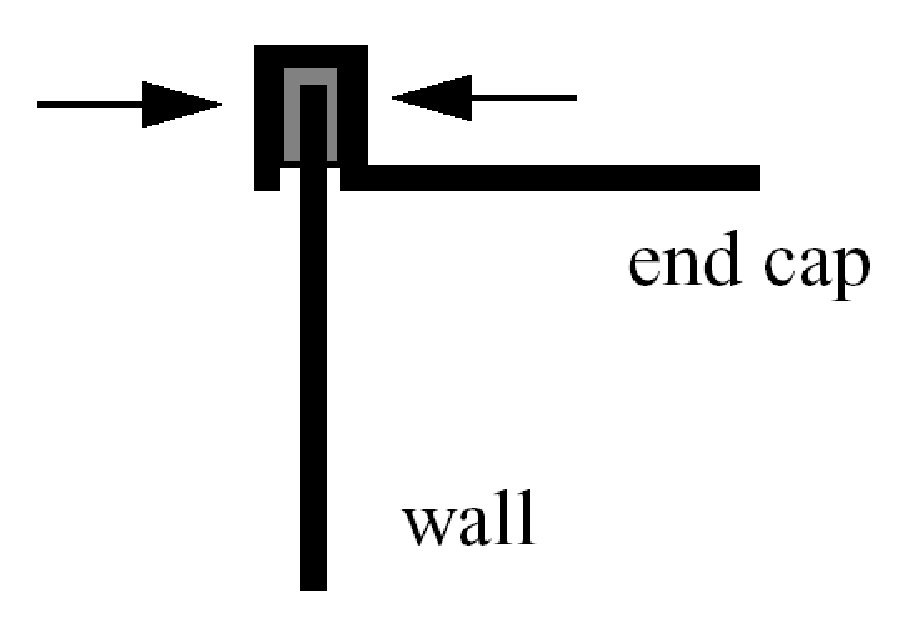
\includegraphics[scale=0.4]{images/end_cap}
  \caption{Container wall-to-end-cap seal}
  \label{additional:figure01}
\end{figure}

For preliminary design purposes, the extra material that would
normally go into the container end cap seals is approximated by
increasing the cut dimensions of the end cap diameters by 12\% and the
height of the container wall by 5\%, and waste associated with
stamping the end caps in a specialized pattern from sheet stock is
estimated as 15\% of the cap area. The equation for the area of the
container materials including waste is

\[
A=2 \times \left(\begin{array}{c}
    \mathtt{end\hbox{ }cap}\\
    \mathtt{waste}\\
    \mathtt{material}\\
    \mathtt{factor}
  \end{array} \right)
\times \left(\begin{array}{c}
    \mathtt{end\hbox{ }cap}\\
    \mathtt{seal}\\
    \mathtt{material}\\
    \mathtt{factor}
  \end{array} \right)
\times \left(\begin{array}{c}
    \mathtt{nominal}\\
    \mathtt{end\hbox{ }cap}\\
    \mathtt{area}
  \end{array} \right)
+ \left(\begin{array}{c}
    \mathtt{container}\\
    \mathtt{wall\hbox{ }seal}\\
    \mathtt{material}\\
    \mathtt{factor}
  \end{array} \right)
\times \left(\begin{array}{c}
    \mathtt{nominal}\\
    \mathtt{container}\\
    \mathtt{wall\hbox{ }area}
  \end{array} \right)
\]

or
\begin{equation}
A=2(1.15)(1.12)\pi\frac{D^2}{4}+(1.05)\pi DH \label{additional:contA}
\end{equation}

where $D$ and $H$ are the diameter and height of the finished product
in units of inches, respectively. The volume of the finished product
is specified to be
\begin{equation}
  V=\pi\frac{D^2H}{4}=(1.1\mathtt{qt})(57.75 \mathtt{in}^3/\mathtt{qt})
  \label{additional:contV}
\end{equation}

The equation for area is the objective function for this problem; it
is to be minimized. The equation for volume is an equality constraint;
it must be satisfied at the conclusion of the optimization problem.
Any combination of $D$ and $H$ that satisfies the volume constraint is
a \textbf{feasible} solution (although not necessarily the optimal
solution) to the area minimization problem, and any combination that
does not satisfy the volume constraint is an \textbf{infeasible}
solution. The area that is a minimum subject to the volume constraint
is the \textbf{optimal} area, and the corresponding values for the
parameters $D$ and $H$ are the optimal parameter values.

It is important that the equations supplied to a numerical
optimization code be limited to generating only physically realizable
values, since an optimizer will not have the capability to
differentiate between meaningful and nonphysical parameter values. It
is often up to the engineer to supply these limits, usually in the
form of parameter bound constraints. For example, by observing the
equations for the area objective function and the volume constraint,
it can be seen that by allowing the diameter, $D$, to become negative,
it is algebraically possible to generate relatively small values for
the area that also satisfy the volume constraint. Negative values for
$D$ are of course physically meaningless. Therefore, to ensure that
the numerically-solved optimization problem remains meaningful, a
bound constraint of $-D \leq 0$ must be included in the optimization
problem statement. A positive value for $H$ is implied since the
volume constraint could never be satisfied if $H$ were negative.
However, a bound constraint of $-H \leq 0$ can be added to the
optimization problem if desired. The optimization problem can then be
stated in a standardized form as
\begin{eqnarray}
\texttt{minimize}   & & 2(1.15)(1.12)\pi\frac{D^2}{4}+(1.05)^2\pi DH\nonumber\\
\texttt{subject to} & & \pi\frac{D^2H}{4}=
  (1.1\mathtt{qt})(57.75 \mathtt{in}^3/\mathtt{qt}) \label{additional:contFH}\\
                    & & -D \leq 0\hbox{, }-H \leq 0\nonumber
\end{eqnarray}

A graphical view of the container optimization test problem appears in
Figure~\ref{additional:figure02}. The 3-D surface defines the area,
$A$, as a function of diameter and height. The curved line that
extends across the surface defines the areas that satisfy the volume
equality constraint, $V$. Graphically, the container optimization
problem can be viewed as one of finding the point along the constraint
line with the smallest 3-D surface height in
Figure~\ref{additional:figure02}. This point corresponds to the
optimal values for diameter and height of the final product.

\begin{figure}
  \centering
  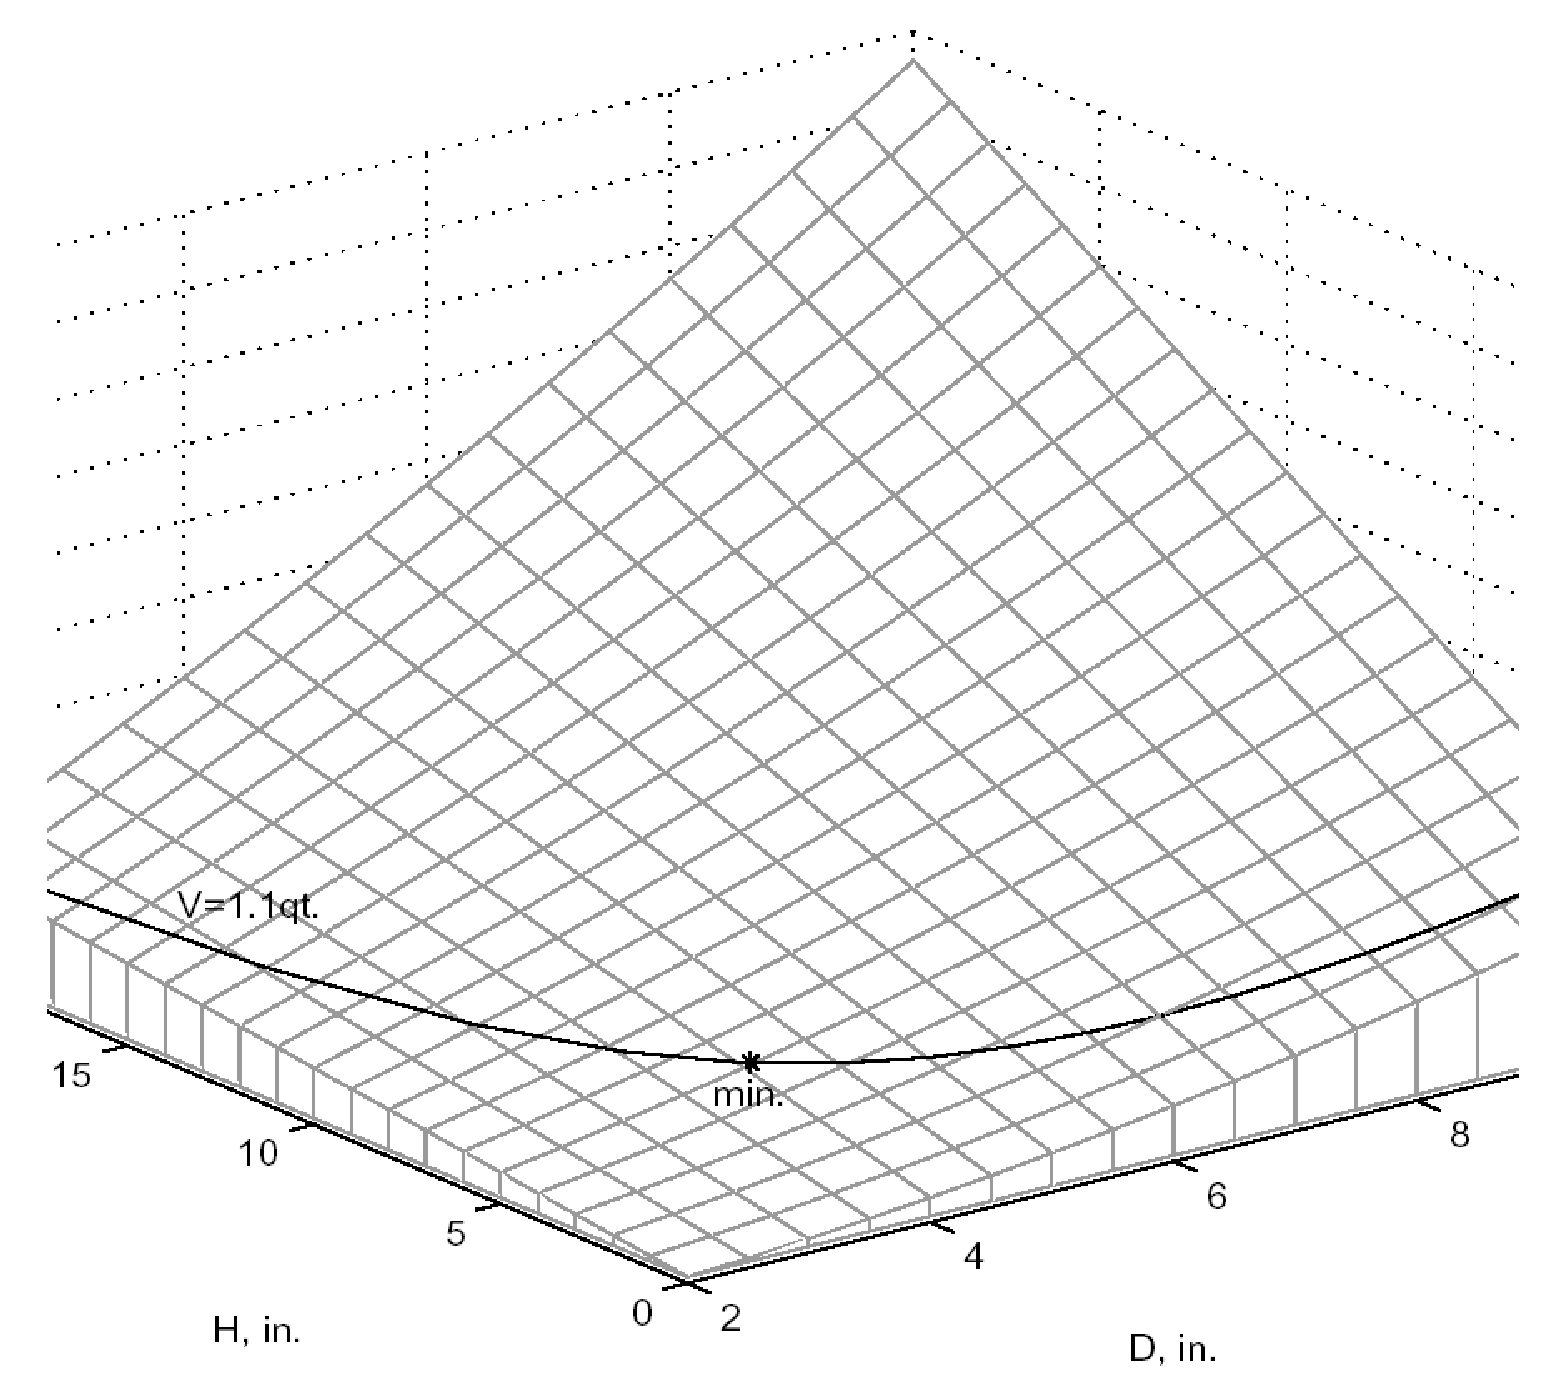
\includegraphics[scale=0.3]{images/graphical_container_opt}
  \caption{A graphical representation of the container optimization
    problem.}
  \label{additional:figure02}
\end{figure}

\subsection{Constrained Gradient Based Optimization}

The input file for this example is named
\texttt{container\_opt\_npsol.in}. The solution to this example
problem is $(H,D)=(4.99,4.03)$, with a minimum area of 98.43
$\mathtt{in}^2$ .

The final report from the Dakota output is as follows:
\begin{small}
\begin{verbatim}
    <<<<< Iterator npsol_sqp completed.
    <<<<< Function evaluation summary: 40 total (40 new, 0 duplicate)
    <<<<< Best parameters          =
                          4.9873894231e+00 H
                          4.0270846274e+00 D
    <<<<< Best objective function  =
                          9.8432498116e+01
    <<<<< Best constraint values   =
                         -9.6301439045e-12
    <<<<< Best data captured at function evaluation 36
    <<<<< Environment execution completed.
    Dakota execution time in seconds:
      Total CPU        =      0.18 [parent =      0.18, child =         0]
      Total wall clock =  0.809126
\end{verbatim}
\label{cont_opt_npsol.out}
\end{small}

% Begin UQ testers

\section{Cantilever}\label{additional:cantilever}

This test problem is adapted from the reliability-based design
optimization literature~\cite{Sue01},~\cite{Wu01} and involves a simple
uniform cantilever beam as shown in Figure~\ref{additional:figure03}.

\begin{figure}[hbp]
  \centering
  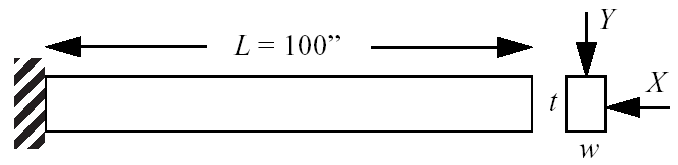
\includegraphics[scale=0.5]{images/cantilever_beam}
  \caption{Cantilever beam test problem.}
  \label{additional:figure03}
\end{figure}

The design problem is to minimize the weight (or, equivalently, the
cross-sectional area) of the beam subject to a displacement constraint
and a stress constraint. Random variables in the problem include the
yield stress $R$ of the beam material, the Young's modulus $E$ of the
material, and the horizontal and vertical loads, $X$ and $Y$, which
are modeled with normal distributions using $N(40000, 2000)$,
$N(2.9E7, 1.45E6)$, $N(500, 100)$, and $N(1000, 100)$, respectively.
Problem constants include $L = 100\mathtt{in}$ and $D_{0} = 2.2535
\mathtt{in}$. The constraints have the following analytic form:
\begin{eqnarray}
\mathtt{stress}&=&\frac{600}{w t^2}Y+\frac{600}{w^2t}X \leq R
  \label{additional:cant}\\
\mathtt{displacement}&=&\frac{4L^3}{E w t}
  \sqrt{\bigg(\frac{Y}{t^2}\bigg)^2+\bigg(\frac{X}{w^2}\bigg)^2}
  \leq D_{0} \nonumber
\end{eqnarray}
or when scaled:
\begin{eqnarray}
  g_{S}&=&\frac{\mathtt{stress}}{R}-1 \leq 0\label{additional:cantscale}\\
  g_{D}&=&\frac{\mathtt{displacement}}{D_{0}}-1 \leq 0\nonumber\\
\end{eqnarray}

{\bf Deterministic Formulation } \\
If the random variables $E$, $R$, $X$, and $Y$ are fixed at their
means, the resulting deterministic design problem can be formulated as
\begin{eqnarray}
\texttt{minimize }   & & f = w t            \nonumber\\
\texttt{subject to } & & g_{S} \leq 0 \label{additional:cantopt}\\
                     & & g_{D} \leq 0       \nonumber\\
                     & & 1.0 \leq w \leq 4.0\nonumber\\
                     & & 1.0 \leq t \leq 4.0\nonumber
\end{eqnarray}

{\bf Stochastic Formulation } \\
If the normal distributions for the random variables $E$, $R$, $X$,
and $Y$ are included, a stochastic design problem can be formulated as
\begin{eqnarray}
\texttt{minimize }   & & f = w t            \nonumber\\
\texttt{subject to } & & \beta_{D} \geq 3   \label{additional:cantouu}\\
                     & & \beta_{S} \geq 3   \nonumber\\
                     & & 1.0 \leq w \leq 4.0\nonumber\\
                     & & 1.0 \leq t \leq 4.0\nonumber
\end{eqnarray}
where a 3-sigma reliability level (probability of failure = 0.00135 if
responses are normally-distributed) is being sought on the scaled
constraints.

\subsection{Constrained Gradient Based Optimization}
The test problem is solved using {\tt cantilever\_opt\_npsol.in}:
\begin{figure}[ht!]
  \centering
  \begin{small}
    \begin{bigbox}
      \verbatimtabinput[8]{cantilever_opt_npsol.in}
    \end{bigbox}
  \end{small}
  \caption{Cantilever Example: the Dakota input file --
see \texttt{Dakota/examples/users/cantilever\_opt\_npsol.in} }
  \label{additional:cant_opt_npsol}
\end{figure}

The deterministic solution is $(w,t)=(2.35,3.33)$ with an objective
function of $7.82$. The final report from the Dakota output is as
follows:
\begin{small}
\begin{verbatim}
    <<<<< Iterator npsol_sqp completed.
    <<<<< Function evaluation summary: 33 total (33 new, 0 duplicate)
    <<<<< Best parameters          =
                          2.3520341271e+00 beam_width
                          3.3262784077e+00 beam_thickness
                          4.0000000000e+04 R
                          2.9000000000e+07 E
                          5.0000000000e+02 X
                          1.0000000000e+03 Y
    <<<<< Best objective function  =
                          7.8235203313e+00
    <<<<< Best constraint values   =
                         -1.6009000260e-02
                         -3.7083558446e-11
    <<<<< Best data captured at function evaluation 31
    <<<<< Environment execution completed.
    Dakota execution time in seconds:
      Total CPU        =       0.03 [parent =   0.027995, child =   0.002005]
      Total wall clock =   0.281375
\end{verbatim}
\end{small}

\subsection{Optimization Under Uncertainty}
Optimization under uncertainty solutions to the
stochastic problem are described in~\cite{Eld02,Eld05,Eld06a}, for
which the solution is $(w,t)=(2.45,3.88)$ with an objective function
of $9.52$. This demonstrates that a more conservative design is
needed to satisfy the probabilistic constraints.

\section{Multiobjective Test Problems}\label{additional:multiobjective}

Multiobjective optimization means that there are two or more
objective functions that you wish to optimize simultaneously. Often
these are conflicting objectives, such as cost and performance. The
answer to a multi-objective problem is usually not a single point.
Rather, it is a set of points called the Pareto front. Each point
on the Pareto front satisfies the Pareto optimality criterion, i.e.,
locally there exists no other feasible vector that would improve some
objective without causing a simultaneous worsening in at least one
other objective. Thus a feasible point $X^\prime$ from which
small moves improve one or more objectives without worsening
any others is not Pareto optimal: it is said to be ``dominated''
and the points along the Pareto front are said to be
``non-dominated''.

Often multi-objective problems are addressed by simply assigning
weights to the individual objectives, summing the weighted objectives,
and turning the problem into a single-objective one which can be
solved with a variety of optimization techniques. While this approach
provides a useful ``first cut'' analysis (and is supported within
Dakota---see Section~\ref{opt:additional:multiobjective}), this
approach has many limitations. The major limitation is that a local
solver with a weighted sum objective will only find one
% optimal solutions if the true Pareto front is nonconvex. %Hogwash!
point on the Pareto front; if one wants to understand
the effects of changing weights, this method can be computationally
expensive. Since each optimization of a single weighted objective
will find only one point on the Pareto front, many
optimizations must be performed to get a good parametric
understanding of the influence of the weights and to achieve a good
sampling of the entire Pareto frontier.

There are three examples that are taken from a multiobjective
evolutionary algorithm (MOEA) test suite described by Van Veldhuizen
et. al. in~\cite{Coe02}. These three examples illustrate the different
forms that the Pareto set may take. For each problem, we describe the
Dakota input and show a graph of the Pareto front. These problems are
all solved with the \texttt{moga} method.  The first example is
discussed in Section~\ref{opt:additional:multiobjective}.  The next
two are discussed below.  Section~\ref{opt:additional:multiobjective}
provide more information on multiobjective optimization.

\subsection{Multiobjective Test Problem 2}\label{additional:multiobjective:problem2}

The second test problem is a case where both $\mathtt{P_{true}}$ and
$\mathtt{PF_{true}}$ are disconnected. $\mathtt{PF_{true}}$ has four
separate Pareto curves. The problem is to simultaneously optimize
$f_1$ and $f_2$ given two input variables, $x_1$ and $x_2$,
where the inputs are bounded by $0 \leq x_{i} \leq 1$, and:
\begin{eqnarray*}
f_1(x) &=& x_1 \\
f_2(x) &=& (1+10x_2) \times \left[1-\bigg(\frac{x_1}{1+10x_2}\bigg)^2-
\frac{x_1}{1+10x_2}\sin(8\pi x_1)\right]
\end{eqnarray*}

The input file for this example is shown in
Figure~\ref{additional:moga2inp}, which references the
\texttt{mogatest2} executable (compiled from
\texttt{Dakota\_Source/test/mogatest2.cpp}) as the simulator. The Pareto
front is shown in Figure~\ref{additional:moga2front}. Note the
discontinuous nature of the front in this example.

\begin{figure}
  \centering
  \begin{bigbox}
    \begin{small}
      \verbatimtabinput[8]{mogatest2.in}
    \end{small}
  \end{bigbox}
  \caption{Dakota input file specifying the use of MOGA on mogatest2 --
see \texttt{Dakota/examples/users/mogatest2.in} }
  \label{additional:moga2inp}
\end{figure}

\begin{figure}
  \centering
  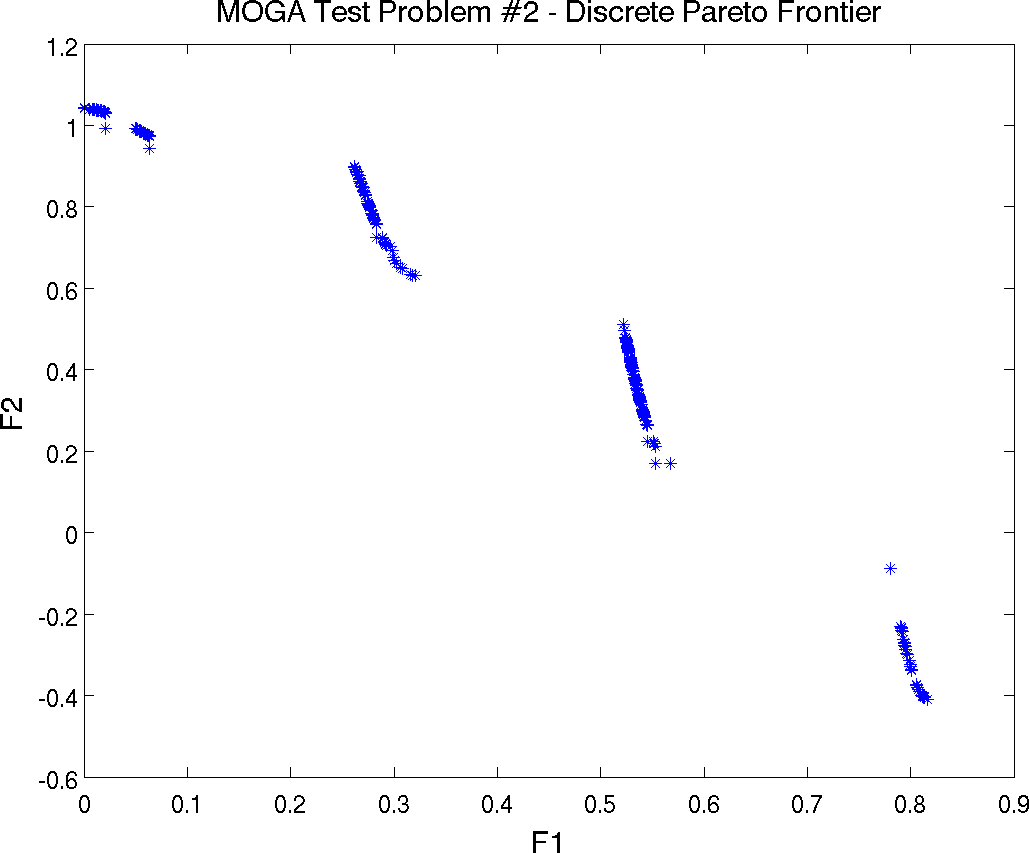
\includegraphics[scale=0.75]{images/dakota_mogatest2_pareto_front}
  \caption{Pareto Front showing Tradeoffs between Function F1 and
    Function F2 for mogatest2}
  \label{additional:moga2front}
\end{figure}

\subsection{Multiobjective Test Problem 3}\label{additional:multiobjective:problem3}

The third test problem is a case where $\mathtt{P_{true}}$ is
disconnected but $\mathtt{PF_{true}}$ is connected. 
% It is called the Srinivas problem in the literature (cite). 
This problem also has two
nonlinear constraints. The problem is to simultaneously optimize
$f_1$ and $f_2$ given two input variables, $x_1$ and $x_2$,
where the inputs are bounded by $-20 \leq x_{i} \leq 20$, and:
\begin{eqnarray*}
f_1(x) &=& (x_1-2)^2+(x_2-1)^2+2 \\
f_2(x) &=& 9x_1-(x_2-1)^2
\end{eqnarray*}

The constraints are:
\begin{eqnarray*}
0 &\leq& x_1^2+x_2^2-225 \\
0 &\leq& x_1-3x_2+10
\end{eqnarray*}

The input file for this example is shown in
Figure~\ref{additional:moga3inp}. It differs from
Figure~\ref{additional:moga2inp} in the variables and responses
specifications, in the use of the \texttt{mogatest3} executable
(compiled from \texttt{Dakota\_Source/test/mogatest3.cpp}) as the simulator, and
in the \texttt{max\_function\_evaluations} and \texttt{mutation\_type}
MOGA controls. The Pareto set is shown in
Figure~\ref{additional:moga3set}. Note the discontinuous nature of the
Pareto set (in the design space) in this example. The Pareto front is
shown in Figure~\ref{additional:moga3front}.
%Again, note the unusual nature of this Pareto example (these figures 
%agree reasonably well with the Srinivas problem results shown in the 
%literature).

\begin{figure}
  \centering
  \begin{bigbox}
    \begin{small}
      \verbatimtabinput[8]{mogatest3.in}
    \end{small}
  \end{bigbox}
  \caption{Dakota input file specifying the use of MOGA on mogatest3 --
see \texttt{Dakota/examples/users/mogatest3.in} }
  \label{additional:moga3inp}
\end{figure}

\begin{figure}
  \centering
  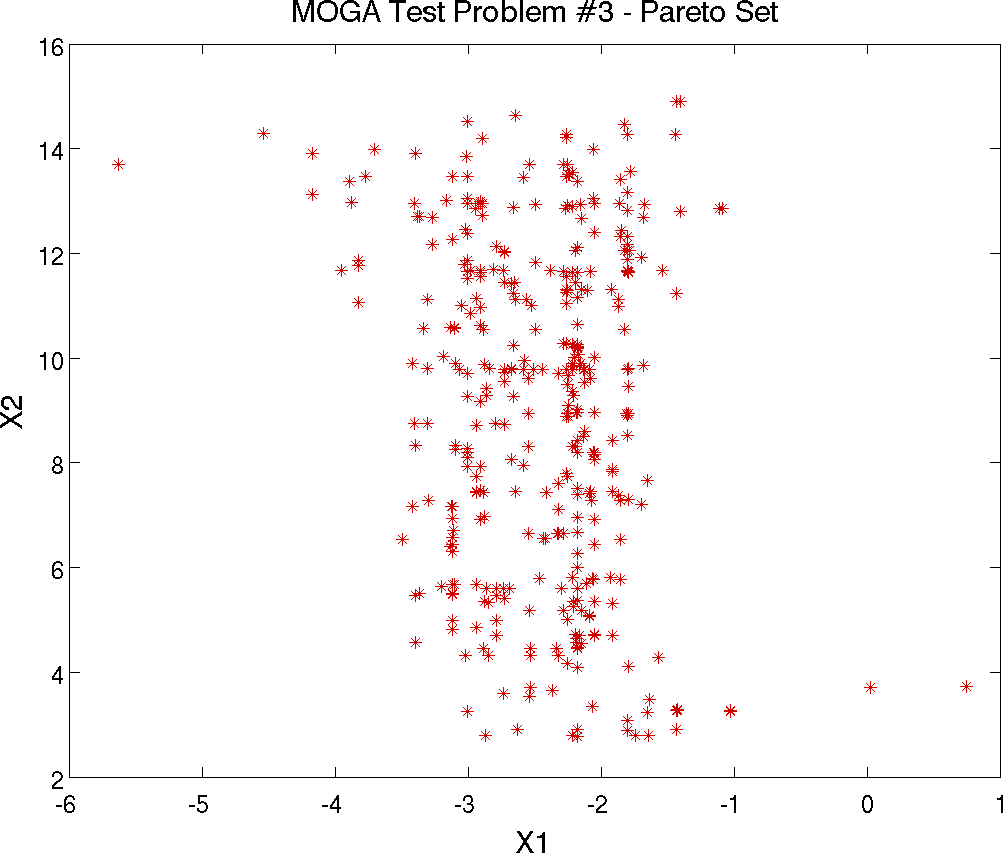
\includegraphics[scale=0.75]{images/dakota_mogatest3_pareto_set}
  \caption{Pareto Set of Design Variables corresponding to the Pareto
    front for mogatest3}
  \label{additional:moga3set}
\end{figure}

\begin{figure}
  \centering
  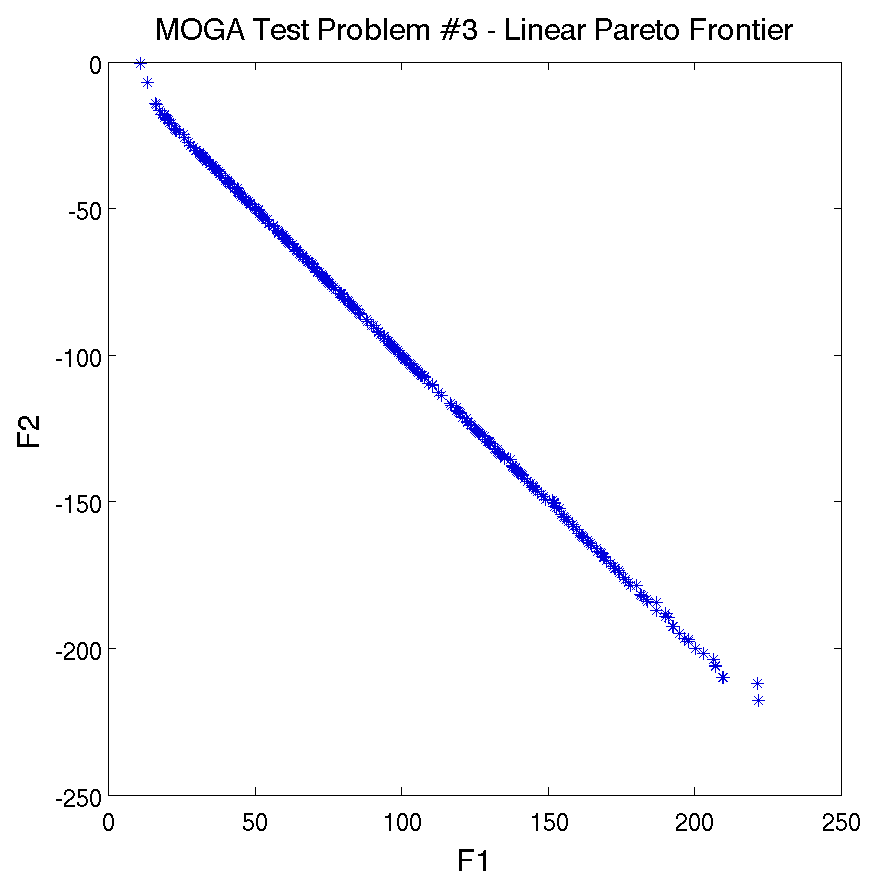
\includegraphics[scale=0.75]{images/dakota_mogatest3_pareto_front}
  \caption{Pareto Front showing Tradeoffs between Function F1 and
    Function F2 for mogatest3}
  \label{additional:moga3front}
\end{figure}

\clearpage
\section{Morris}\label{additional:morris}

Morris~\cite{Mor91} includes a screening design test problem with a
single-output analytical test function. The output depends on 20
inputs with first- through fourth-order interaction terms, some having
large fixed coefficients and others small random coefficients. Thus
the function values generated depend on the random number generator
employed in the function evaluator. The computational model is:

\begin{align*}
y = &\;\beta_0 + \sum_{i=1}^{20}{\beta_i w_i} + \sum_{i<j}^{20}{\beta_{i,j} w_i w_j} + \sum_{i<j<l}^{20}{\beta_{i,j,l} w_i w_j w_l} \\
    &+  \sum_{i<j<l<s}^{20}{\beta_{i,j,l,s} w_i w_j w_l w_s},
\end{align*}
where $w_i = 2(x_i-0.5)$ except for $i=3, 5, \mbox{ and } 7$, where $w_i=2(1.1x_i/(x_i+0.1) - 0.5)$. Large-valued coefficients are assigned as 
\begin{align*}
&\beta_i = +20 & &i=1,\ldots,10; \;&\beta_{i,j} = -15& &i,j = 1, \ldots, 6; \\
&\beta_{i,j,l} = -10& &i,j,l=1,\ldots,5; \;&\beta_{i,j,l,s} = +5& &i,j,l,s = 1, \ldots, 4.
\end{align*}
The remaining first- and second-order coefficients $\beta_i$ and
$\beta_{i,j}$, respectively, are independently generated from a
standard normal distribution (zero mean and unit standard deviation);
the remaining third- and fourth-order coefficients are set to zero.

Examination of the test function reveals that one should be able to
conclude the following (stated and verified computationally
in~\cite{Sal04}) for this test problem:
\begin{enumerate}
\item the first ten factors are important;
\item of these, the first seven have significant effects involving
      either interactions or curvatures; and
\item the other three are important mainly because of their first-order
      effect.
\end{enumerate}

\subsection{Morris One-at-a-Time Sensitivity Study}

The dakota input {\tt morris\_ps\_moat.in} exercises
the MOAT algorithm described in Section~\ref{dace:psuade} on the
Morris problem. The Dakota output obtained is shown in
Figures~\ref{FIG:moat:out_preamble} and~\ref{FIG:moat:out_results}.
\begin{figure}[ht!]
\centering
\begin{bigbox}
\begin{small}
\begin{verbatim}
Running MPI executable in serial mode.
Dakota version 6.0 release.
Subversion revision xxxx built May ...
Writing new restart file dakota.rst
gradientType = none
hessianType = none

>>>>> Executing environment.

>>>>> Running psuade_moat iterator.

PSUADE DACE method = psuade_moat Samples = 84 Seed (user-specified) = 500
            Partitions = 3 (Levels = 4)
\end{verbatim}
\end{small}
\end{bigbox}
\caption[Dakota initialization output for PSUADE
MOAT.]{\label{FIG:moat:out_preamble} Dakota initialization output for
the PSUADE MOAT method on the Morris test problem showing the study
parameters.}
\end{figure}
\begin{figure}[ht!]
\centering
\begin{bigbox}
\begin{small}
\begin{verbatim}
>>>>>> PSUADE MOAT output for function 0:

*************************************************************
*********************** MOAT Analysis ***********************
-------------------------------------------------------------
Input   1 (mod. mean & std) =   9.5329e+01   9.0823e+01 
Input   2 (mod. mean & std) =   6.7297e+01   9.5242e+01 
Input   3 (mod. mean & std) =   1.0648e+02   1.5479e+02 
Input   4 (mod. mean & std) =   6.6231e+01   7.5895e+01 
Input   5 (mod. mean & std) =   9.5717e+01   1.2733e+02 
Input   6 (mod. mean & std) =   8.0394e+01   9.9959e+01 
Input   7 (mod. mean & std) =   3.2722e+01   2.7947e+01 
Input   8 (mod. mean & std) =   4.2013e+01   7.6090e+00 
Input   9 (mod. mean & std) =   4.1965e+01   7.8535e+00 
Input  10 (mod. mean & std) =   3.6809e+01   3.6151e+00 
Input  11 (mod. mean & std) =   8.2655e+00   1.0311e+01 
Input  12 (mod. mean & std) =   4.9299e+00   7.0591e+00 
Input  13 (mod. mean & std) =   3.5455e+00   4.4025e+00 
Input  14 (mod. mean & std) =   3.4151e+00   2.4905e+00 
Input  15 (mod. mean & std) =   2.5143e+00   5.5168e-01 
Input  16 (mod. mean & std) =   9.0344e+00   1.0115e+01 
Input  17 (mod. mean & std) =   6.4357e+00   8.3820e+00 
Input  18 (mod. mean & std) =   9.1886e+00   2.5373e+00 
Input  19 (mod. mean & std) =   2.4105e+00   3.1102e+00 
Input  20 (mod. mean & std) =   5.8234e+00   7.2403e+00 
<<<<< Function evaluation summary: 84 total (84 new, 0 duplicate)
\end{verbatim}
\end{small}
\end{bigbox}
\caption[Dakota analysis output for PSUADE
MOAT.]{\label{FIG:moat:out_results} Dakota analysis output for the
PSUADE MOAT method on the Morris problem showing the modified
mean and standard deviation of the elementary effect corresponding to
each input factor.}
\end{figure}
The MOAT analysis output reveals that each of the desired observations
can be made for the test problem. These are also reflected in
Figure~\ref{FIG:mustar_sigma}. The modified mean (based on averaging
absolute values of elementary effects) shows a clear difference in
inputs 1--10 as compared to inputs 11--20. The standard deviation of
the (signed) elementary effects indicates correctly that inputs 1--7
have substantial interaction-based or nonlinear effect on the output,
while the others have less. While some of inputs 11--20 have
nontrivial values of $\sigma$, their relatively small modified means
$\mu^*$ indicate they have little overall influence.

\begin{figure}[ht!]
\centering
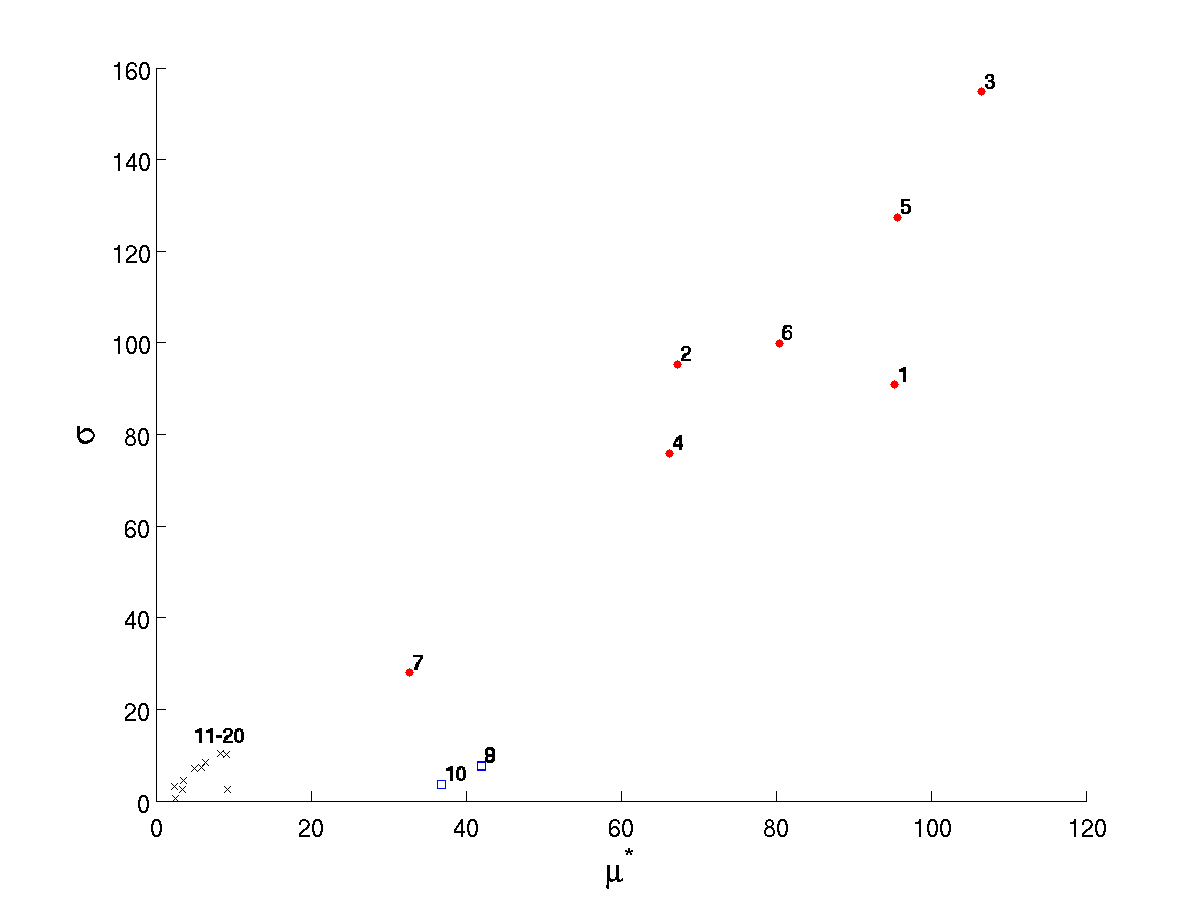
\includegraphics[width=\textwidth]{images/moat_mustar_sigma}
\caption{\label{FIG:mustar_sigma} Standard deviation of elementary
effects plotted against modified mean for Morris for each of 20
inputs. Red circles 1--7 correspond to inputs having interactions or
nonlinear effects, blue squares 8--10 indicate those with mainly
linear effects, and black Xs denote insignificant inputs.}
\end{figure}

\clearpage
\section{Test Problems for Reliability Analyses}\label{additional:reliabilityproblems}
This section includes several test problems and examples related to 
reliability analyses. {\bf These are NOT included in the {\tt Dakota/examples/users} 
directory, but are in the {\tt Dakota/test} directory.}


\subsection{Log Ratio}\label{additional:logratio}

This test problem, mentioned previously in
Section~\ref{uq:reliability:ex}, has a limit state function defined by
the ratio of two lognormally-distributed random variables.
\begin{equation}
g({\bf x}) = \frac{x_1}{x_2}
\end{equation}
The distributions for both $x_1$ and $x_2$ are Lognormal(1, 0.5) with
a correlation coefficient between the two variables of 0.3.

{\bf Reliability Analyses} \\

First-order and second-order reliability analysis (FORM and SORM) are performed in the
\texttt{logratio\_uq\_reliability.in} in the {\tt Dakota/examples/users}
 directory and \texttt{dakota\_logratio\_taylor2.in} in directory 
{\tt Dakota/test}.

For the reliability index approach (RIA),
24 response levels (.4, .5, .55,
.6, .65, .7, .75, .8, .85, .9, 1, 1.05, 1.15, 1.2, 1.25, 1.3, 1.35,
1.4, 1.5, 1.55, 1.6, 1.65, 1.7, and 1.75) are mapped into the
corresponding cumulative probability levels. For performance measure approach (PMA), these 24
probability levels (the fully converged results from RIA FORM) are
mapped back into the original response levels.
Figure~\ref{fig:log_ratio_cdf} overlays the computed CDF values for a
number of first-order reliability method variants as well as a Latin
Hypercube reference solution of $10^6$ samples.
\begin{figure}[hbp]
\centering
\centerline{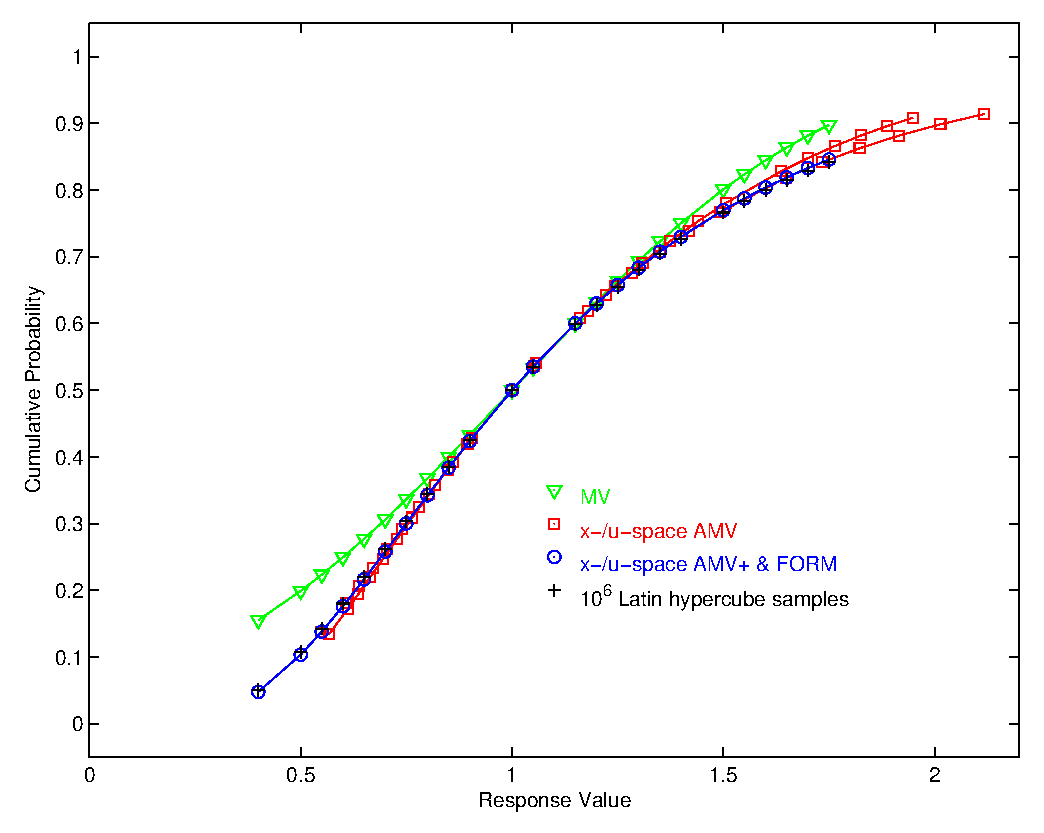
\includegraphics[scale=0.5]{images/log_ratio_cdf_ria}
            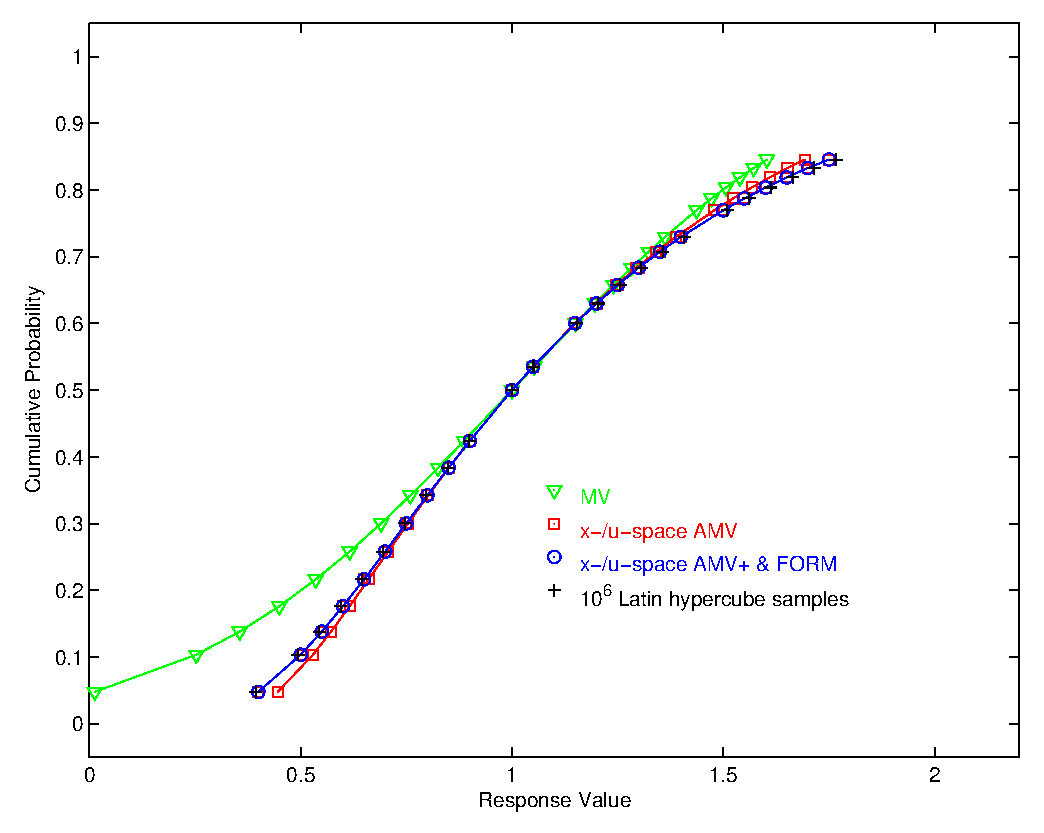
\includegraphics[scale=0.5]{images/log_ratio_cdf_pma}}
(a) RIA methods\hspace{2.5in}(b) PMA methods
\caption{Lognormal ratio cumulative distribution function, RIA/PMA methods.}
\label{fig:log_ratio_cdf}
\end{figure}

\subsection{Steel Section}\label{additional:steel_section}

This test problem is used extensively in~\cite{Hal00}. It involves a
W16x31 steel block of A36 steel that must carry an applied
deterministic bending moment of 1140 kip-in. For Dakota, it has been
used as a code verification test for second-order integrations in
reliability methods. The limit state function is defined as:
\begin{equation}
g({\bf x}) = F_y Z - 1140
\end{equation}
where $F_y$ is Lognormal(38., 3.8), $Z$ is Normal(54., 2.7), and the
variables are uncorrelated.

The \texttt{Dakota/test/dakota\_steel\_section.in} input file computes
a first-order CDF probability of $p(g \leq 0.)$ = 1.297e-07 and a
second-order CDF probability of $p(g \leq 0.)$ = 1.375e-07. This
second-order result differs from that reported in~\cite{Hal00}, since
Dakota uses the Nataf nonlinear transformation to u-space (see MPP
Search Methods block in Reliability Methods chapter of Dakota Theory
Manual~\cite{TheoMan}) and \cite{Hal00} uses a linearized
transformation.

\subsection{Portal Frame}\label{additional:portal_frame}


This test problem is taken from~\cite{Tve90,Hon99}. It involves a
plastic collapse mechanism of a simple portal frame. It also has been
used as a verification test for second-order integrations in 
reliability methods. The limit state function is defined as:
\begin{equation}
g({\bf x}) = x_1 + 2 x_2 + 2 x_3 + x_4 - 5 x_5 - 5 x_6
\end{equation}
where $x_1 - x_4$ are Lognormal(120., 12.), $x_5$ is Lognormal(50.,
15.), $x_6$ is Lognormal(40., 12.), and the variables are uncorrelated.

While the limit state is linear in x-space, the nonlinear
transformation of lognormals to u-space induces curvature. The
\texttt{Dakota/test/dakota\_portal\_frame.in} input file computes a
first-order CDF probability of $p(g \leq 0.)$ = 9.433e-03 and a
second-order CDF probability of $p(g \leq 0.)$ = 1.201e-02. These
results agree with the published results from the literature.

\subsection{Short Column}\label{additional:short_column}

This test problem involves the plastic analysis and design of a short
column with rectangular cross section (width $b$ and depth $h$) having
uncertain material properties (yield stress $Y$) and subject to
uncertain loads (bending moment $M$ and axial force $P$)~\cite{Kus97}.
The limit state function is defined as:
\begin{equation}
g({\bf x}) = 1 - \frac{4M}{b h^2 Y} - \frac{P^2}{b^2 h^2 Y^2}
\end{equation}

The distributions for $P$, $M$, and $Y$ are Normal(500, 100),
Normal(2000, 400), and Lognormal(5, 0.5), respectively, with a
correlation coefficient of 0.5 between $P$ and $M$ (uncorrelated
otherwise). The nominal values for $b$ and $h$ are 5 and 15,
respectively.

{\bf Reliability Analyses} \\

First-order and second-order reliability analysis are performed in the
\texttt{dakota\_short\_column.in} and \\
\texttt{dakota\_short\_column\_taylor2.in} input files in 
{\tt Dakota/test}. For RIA, 43 response levels (-9.0, -8.75,
-8.5, -8.0, -7.75, -7.5, -7.25, -7.0, -6.5, -6.0, -5.5, -5.0, -4.5,
-4.0, -3.5, -3.0, -2.5, -2.0, -1.9, -1.8, -1.7, -1.6, -1.5, -1.4,
-1.3, -1.2, -1.1, -1.0, -0.9, -0.8, -0.7, -0.6, -0.5, -0.4, -0.3,
-0.2, -0.1, 0.0, 0.05, 0.1, 0.15, 0.2, 0.25) are mapped into the
corresponding cumulative probability levels. For PMA, these 43
probability levels (the fully converged results from RIA FORM) are
mapped back into the original response levels.
Figure~\ref{fig:short_col_cdf} overlays the computed CDF values for
several first-order reliability method variants as well as a Latin
Hypercube reference solution of $10^6$ samples.

\begin{figure}
\centering
\centerline{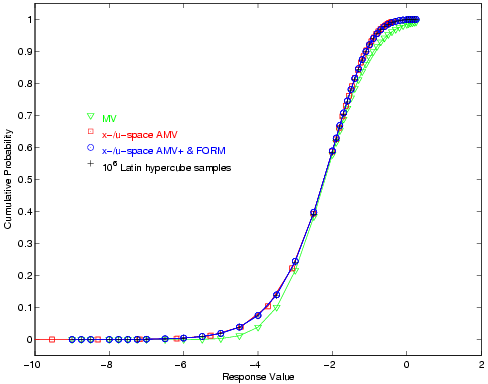
\includegraphics[scale=0.5]{images/short_col_cdf_ria}
            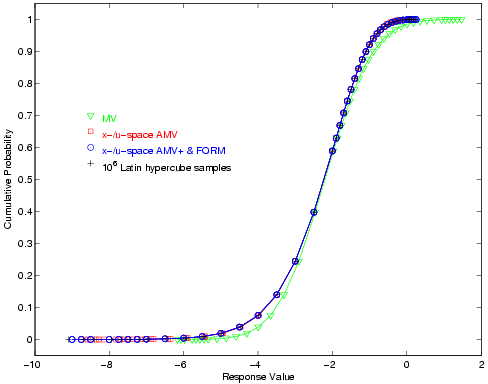
\includegraphics[scale=0.5]{images/short_col_cdf_pma}}
(a) RIA methods\hspace{2.75in}(b) PMA methods
\caption{Short column cumulative distribution function, RIA/PMA methods.}
\label{fig:short_col_cdf}
\end{figure}

{\bf Reliability-Based Design Optimization} \\

The short column test problem is also amenable to Reliability-Based Design Optimization (RBDO). An
objective function of cross-sectional area and a target reliability
index of 2.5 (cumulative failure probability $p(g \le 0) \le 0.00621$) 
are used in the design problem:
\begin{eqnarray}
\min       & & bh \nonumber \\
{\rm s.t.} & & \beta \geq 2.5 \nonumber \\
           & &  5.0 \leq b \leq 15.0 \nonumber \\
           & & 15.0 \leq h \leq 25.0
\end{eqnarray}
As is evident from the UQ results shown in
Figure~\ref{fig:short_col_cdf}, the initial design of $(b, h) = (5,
15)$ is infeasible and the optimization must add material to obtain
the target reliability at the optimal design $(b, h) = (8.68, 25.0)$.
Simple bi-level, fully analytic bi-level, and sequential RBDO methods
are explored in inputs files \\
\texttt{dakota\_rbdo\_short\_column.in},
\texttt{dakota\_rbdo\_short\_column\_analytic.in}, and\\
\texttt{dakota\_rbdo\_short\_column\_trsb.in}, with results as
described in~\cite{Eld05,Eld06a}. These files are located in {\tt Dakota/test}.

\subsection{Steel Column}\label{additional:steel_column}

This test problem involves the trade-off between cost and
reliability for a steel column~\cite{Kus97}. The cost is defined as
\begin{equation}
Cost = b d + 5 h
\end{equation}
where $b$, $d$, and $h$ are the means of the flange breadth, flange
thickness, and profile height, respectively. Nine uncorrelated random
variables are used in the problem to define the yield stress $F_s$
(lognormal with $\mu/\sigma$ = 400/35 MPa), dead weight load $P_1$
(normal with $\mu/\sigma$ = 500000/50000 N), variable load $P_2$
(gumbel with $\mu/\sigma$ = 600000/90000 N), variable load $P_3$
(gumbel with $\mu/\sigma$ = 600000/90000 N), flange breadth $B$
(lognormal with $\mu/\sigma$ = $b$/3 mm), flange thickness $D$
(lognormal with $\mu/\sigma$ = $d$/2 mm), profile height $H$
(lognormal with $\mu/\sigma$ = $h$/5 mm), initial deflection $F_0$
(normal with $\mu/\sigma$ = 30/10 mm), and Young's modulus $E$ (Weibull
with $\mu/\sigma$ = 21000/4200 MPa). The limit state has the
following analytic form:
\begin{equation}
g = F_s - P \left( \frac{1}{2 B D} + 
\frac{F_0}{B D H} \frac{E_b}{E_b - P} \right)\\
\end{equation}
where
\begin{eqnarray}
P   & = & P_1 + P_2 + P_3 \\
E_b & = & \frac{\pi^2 E B D H^2}{2 L^2}
\end{eqnarray}
and the column length $L$ is 7500 mm.

This design problem (\texttt{dakota\_rbdo\_steel\_column.in} in
\texttt{Dakota/test}) demonstrates design variable insertion into
random variable distribution parameters through the design of the mean
flange breadth, flange thickness, and profile height. The RBDO
formulation maximizes the reliability subject to a cost constraint:
\begin{eqnarray}
{\rm maximize }   & & \beta                   \nonumber \\
{\rm subject to } & & Cost  \leq 4000.       \nonumber \\
                  & & 200.0 \leq b \leq 400.0 \\
                  & &  10.0 \leq d \leq  30.0 \nonumber \\
                  & & 100.0 \leq h \leq 500.0 \nonumber
\end{eqnarray}
which has the solution ($b$, $d$, $h$) = (200.0, 17.50, 100.0) with a
maximal reliability of 3.132.

